\section{Improved Algorithm}

The improved algorithm focuses on the selection of cliques based on the smallest degree nodes and uses a theorem to prune the search space efficiently.

The primary improvement lies in selecting cliques starting with nodes that have the smallest degree, \( \deg(v) \), in the entire graph.
\begin{theorem}
    \label{thm:pruning_theorem} % Label for referencing
    If
    \[
        f(S) < 1 - \frac{\deg(v) (1 - \alpha)}{(|S| - 1) \alpha}
    \]
    for any \( v \in S \), then none of \( S \)'s supersets can be an \( \alpha \)-clique.
\end{theorem}

\paragraph{Pruning Mechanism Using Theorem}
The pruning mechanism is governed by the ~\autoref{thm:pruning_theorem} that sets a condition on when a set \( S \) and its supersets can be classified as non-\( \alpha \)-cliques. For effective pruning:
\begin{itemize}
    \item The condition must hold more frequently.
    \item The upper bound on the right-hand side (RHS) of the theorem must be maximized.
\end{itemize}
Maximizing the RHS upper bound involves minimizing the negative term associated with \( \deg(v) \). Therefore, iterating over nodes from the smallest to largest degree makes the pruning happen as often as possible.

\paragraph{Illustration}
A visual representation of the improvement is shown in  ~\autoref{fig:improved_algorithm}. In the graph, the differing values tested candidates per alpha, show the computation performance of the improved algorithm. For smaller alphas, the effect is more pronounced, but even for the alpha 0.8, the improved algorithm does 47 comparisons less. With alpha reaching 1, there is no difference with the improved and traditional algorithm. This happens, since the RHS of the theorem will become always 1.

\begin{table}[h]
    \centering
    \begin{tabular}{ccc}
        \hline
        Alpha & Basic Algorithm & Improved Algorithm \\
        \hline
        0.5   & 1613            & 1471               \\
        0.6   & 1261            & 1127               \\
        0.7   & 1006            & 902                \\
        0.8   & 621             & 574                \\
        \hline
    \end{tabular}
    \caption{Exact values of tested candidates per alpha}
\end{table}


\paragraph{Impact of Graph Size on \(\alpha\)}
For future research, the effect of the size of the graph might affect the number of candidates tested. Possbily, in larger graphs, the impact of the improved pruning algorithm, might save more tested candidates.

\begin{figure}[h]
    \centering
    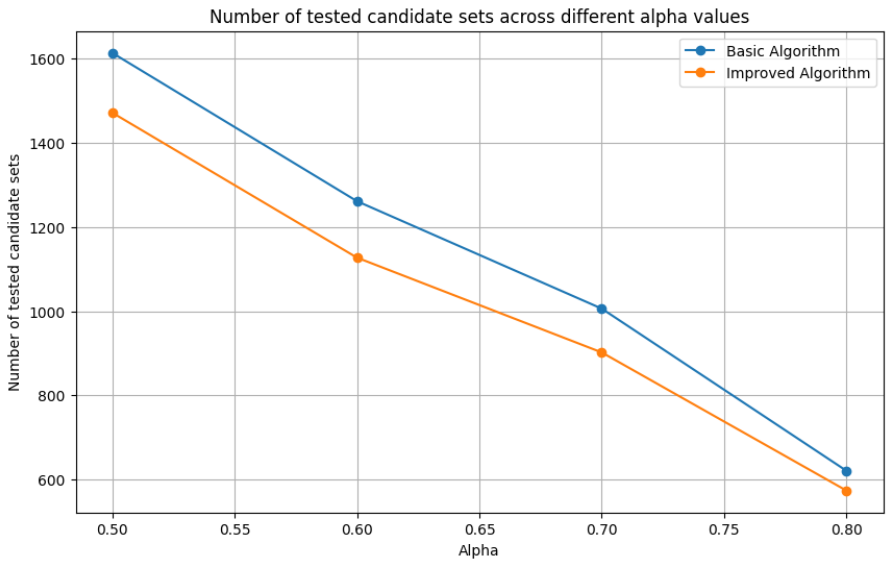
\includegraphics[width=0.8\textwidth]
    {figures/improved_algorithm.png}
    \caption{Different alphas}
    \label{fig:improved_algorithm}
\end{figure}
